% A Readymade beamer presentation template
% Version 1.1
% Relase date: May 2, 2010
% Released at http://www.stattler.com
% by Rifat Jahan

\documentclass{beamer}
%\usecolortheme[named=green]{structure}
\mode<presentation> {
\usetheme{Madrid} % My favorite!
%\usetheme{Boadilla} % Pretty neat, soft color.
%\usetheme{default}
%\usetheme{Warsaw}
%\usetheme{Bergen} % This template has nagivation on the left
%\usetheme{Frankfurt} % Similar to the default with an extra region at the top.
%\usecolortheme{seahorse} % Simple and clean template
%\usetheme{Darmstadt} % not so good
% Uncomment the following line if you want page numbers and using Warsaw theme
% \setbeamertemplate{footline}[page number]
%\setbeamercovered{transparent}
\setbeamercovered{invisible}
% To remove the navigation symbols from the bottom of slides%
\setbeamertemplate{navigation symbols}{} 
}

\usepackage{graphicx}
%\usepackage{bm} 
% For typesetting bold math (not \mathbold)
%\logo{\includegraphics[height=0.6cm]{yourlogo.eps}}

\title[Subspaces]{Face Recognition in Subspaces}

\author{Josh Klontz}
%\institute[U of X]
%{
%University of [...] \\
%\medskip
%{\emph{email@domain.ca}}
%}
\date{\today}
% \today will show current date. 
% Alternatively, you can specify a date.

\begin{document}

\begin{frame}
\titlepage
\end{frame}

\section{Introdution}
\begin{frame}
\frametitle{Works Covered}
\begin{block}{Bayesian face recognition}
Moghaddam, Baback, Tony Jebara, and Alex Pentland. "Bayesian face recognition." Pattern Recognition 33.11 (2000): 1771-1782.
\end{block}
\pause
\begin{block}{Probabilistic models for inference about identity}
Li, Peng, et al. "Probabilistic models for inference about identity." Pattern Analysis and Machine Intelligence, IEEE Transactions on 34.1 (2012): 144-157.
\end{block}
\pause
\begin{block}{Bayesian Face Revisited: A Joint Formulation}
Chen, Dong, et al. "Bayesian Face Revisited: A Joint Formulation."
\end{block}
\end{frame}

\section{Bayesian face recognition}
\begin{frame}
\frametitle{Bayesian face recognition}
\begin{block}{Abstract}
\begin{itemize}
\item \emph{Probabilistic} measure of similarity.
\pause
\item Replace costly \emph{nonlinear} (on-line) computation of Bayesian similarity measure with inexpensive \emph{linear} (off-line) subspace projections and Euclidean norms.
\pause
\item Top performer in 1996 \emph{FERET} face recognition competition.
\end{itemize}
\end{block}
\end{frame}

\begin{frame}
\frametitle{A Bayesian approach}
\begin{block}{Previous Work}
Rely on similarity metrics based on Euclidean distance or normalized correlation.
\pause
Also known as:
\begin{itemize}
\item Template matching
\item Nearest-neighbor-based recognition
\end{itemize}
\end{block}
\pause
\begin{block}{Proposed Approach}
\emph{Probabilistic} similarity measure
\pause
\begin{align}
\Delta& = I_1 - I_2 \\
\Omega_I& \equiv \text{Intrapersonal variations (\emph{same} individual)} \\
\Omega_E& \equiv \text{Extrapersonal variations (\emph{different} individuals)} \\
S(I_1,I_2)& = P(\Delta \in \Omega_I) = P(\Omega_I | \Delta)
\end{align}
\end{block}
\end{frame}

\begin{frame}
\frametitle{Probabilistic similarity measures}
\begin{block}{Bayes Rule}
\begin{equation}
\begin{split}
S(I_1,I_2)& = P(\Omega_I | \Delta) \\
& = \frac{P(\Delta|\Omega_I)P(\Omega_I)}{P(\Delta|\Omega_I)P(\Omega_I)+P(\Delta|\Omega_E)P(\Omega_E)}\equiv \text{MAP} \\
& \approx P(\Delta|\Omega_I)\equiv \text{ML}
\end{split}
\end{equation}
\end{block}
\pause
\begin{block}{Learning Problem}
\begin{itemize}
\item Estimate $P(\Delta|\Omega_I)$ and $P(\Delta|\Omega_E)$ from training data.
\pause
\item Assume both classes are Gaussian-distributed.
\pause
\item \emph{Note:} Bayesian formulation casts the standard face recognition task (essentially an $M$-ary classification problem for $M$ individuals) into a \emph{binary} pattern classification problem with $\Omega_I$ and $\Omega_E$.
\end{itemize}
\end{block}
\end{frame}

\begin{frame}
\frametitle{Subspace density estimation}
\begin{block}{Observations}
\begin{itemize}
\item Intensity difference vector is very high-dimensional: $\Delta \in \mathbb{R}^N \approx O(10^4)$.
\pause
\item Insufficient training examples to compute second-order statistics.
\pause
\item Formidable computational cost even if it was possible.
\pause
\item \emph{Intrinsic} dimensionality of $\Delta$ likely to be significantly smaller.
\end{itemize}
\end{block}
\pause
\begin{block}{Solution}
Approximate $\Delta$ in a lower dimensional PCA subspace: $\Delta^\prime \in \mathbb{R}^M$ such that $M << N$.
\end{block}
\end{frame}

\begin{frame}
\frametitle{Subspace Projection}
\begin{figure}[H]
\centering
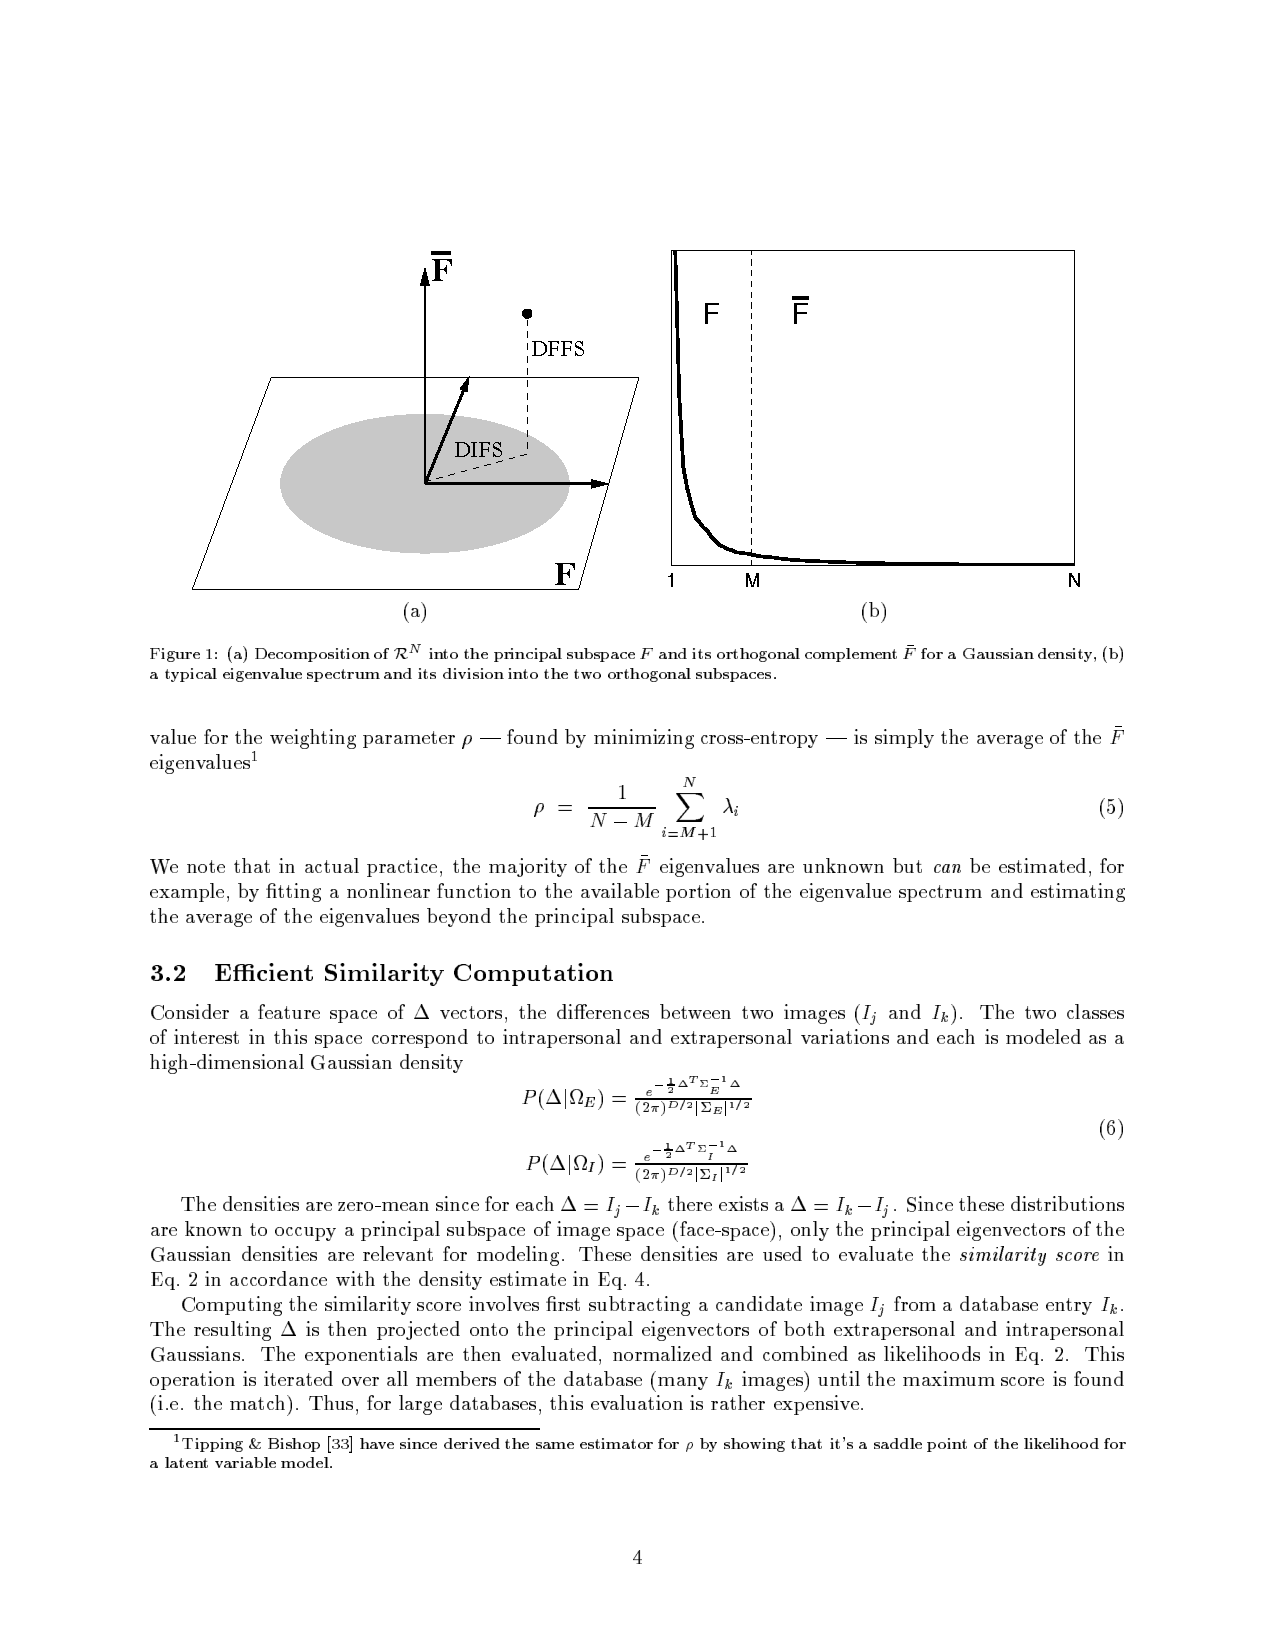
\includegraphics[width=\textwidth, trim=1in 6.4in 1in 1.6in, clip]{Moghaddam6}
\end{figure}
\end{frame}

\begin{frame}
\frametitle{Subspace density estimation}
\begin{block}{Solution details}
Learn subspaces for both $P(\Delta|\Omega_I)$ and $P(\Delta|\Omega_E)$.
\pause
Then approximate $P(\Delta|\Omega)$ with the following observation:
\begin{equation}
\begin{split}
P(\Delta|\Omega)& = P_f(\Delta|\Omega)P_{\bar{f}}(\Delta|\Omega) \\
& \approx P_f(\Delta|\Omega)\hat{P}_{\bar{f}}(\Delta|\Omega) \\
& = \left[\exp\frac{-\frac{1}{2}\sum_{i=1}^My_i^2/\lambda_i}{(2\pi)^{M/2}\prod_{i=1}^M\lambda_i^{1/2}}\right]\left[\frac{\exp(-\epsilon^2(\Delta)/2p)}{(2\pi p)^{(N-M)/2}}\right] \\
\end{split}
\end{equation}
\pause
where
\begin{align}
\epsilon^2(\Delta)& = \text{Residual Reconstruction Error} = \text{DFFS} \\
p& = \frac{1}{N-M}\sum_{i=M+1}^N\lambda_i
\end{align}
\end{block}
\end{frame}

\begin{frame}
\frametitle{Visualization}
\begin{figure}[H]
\centering
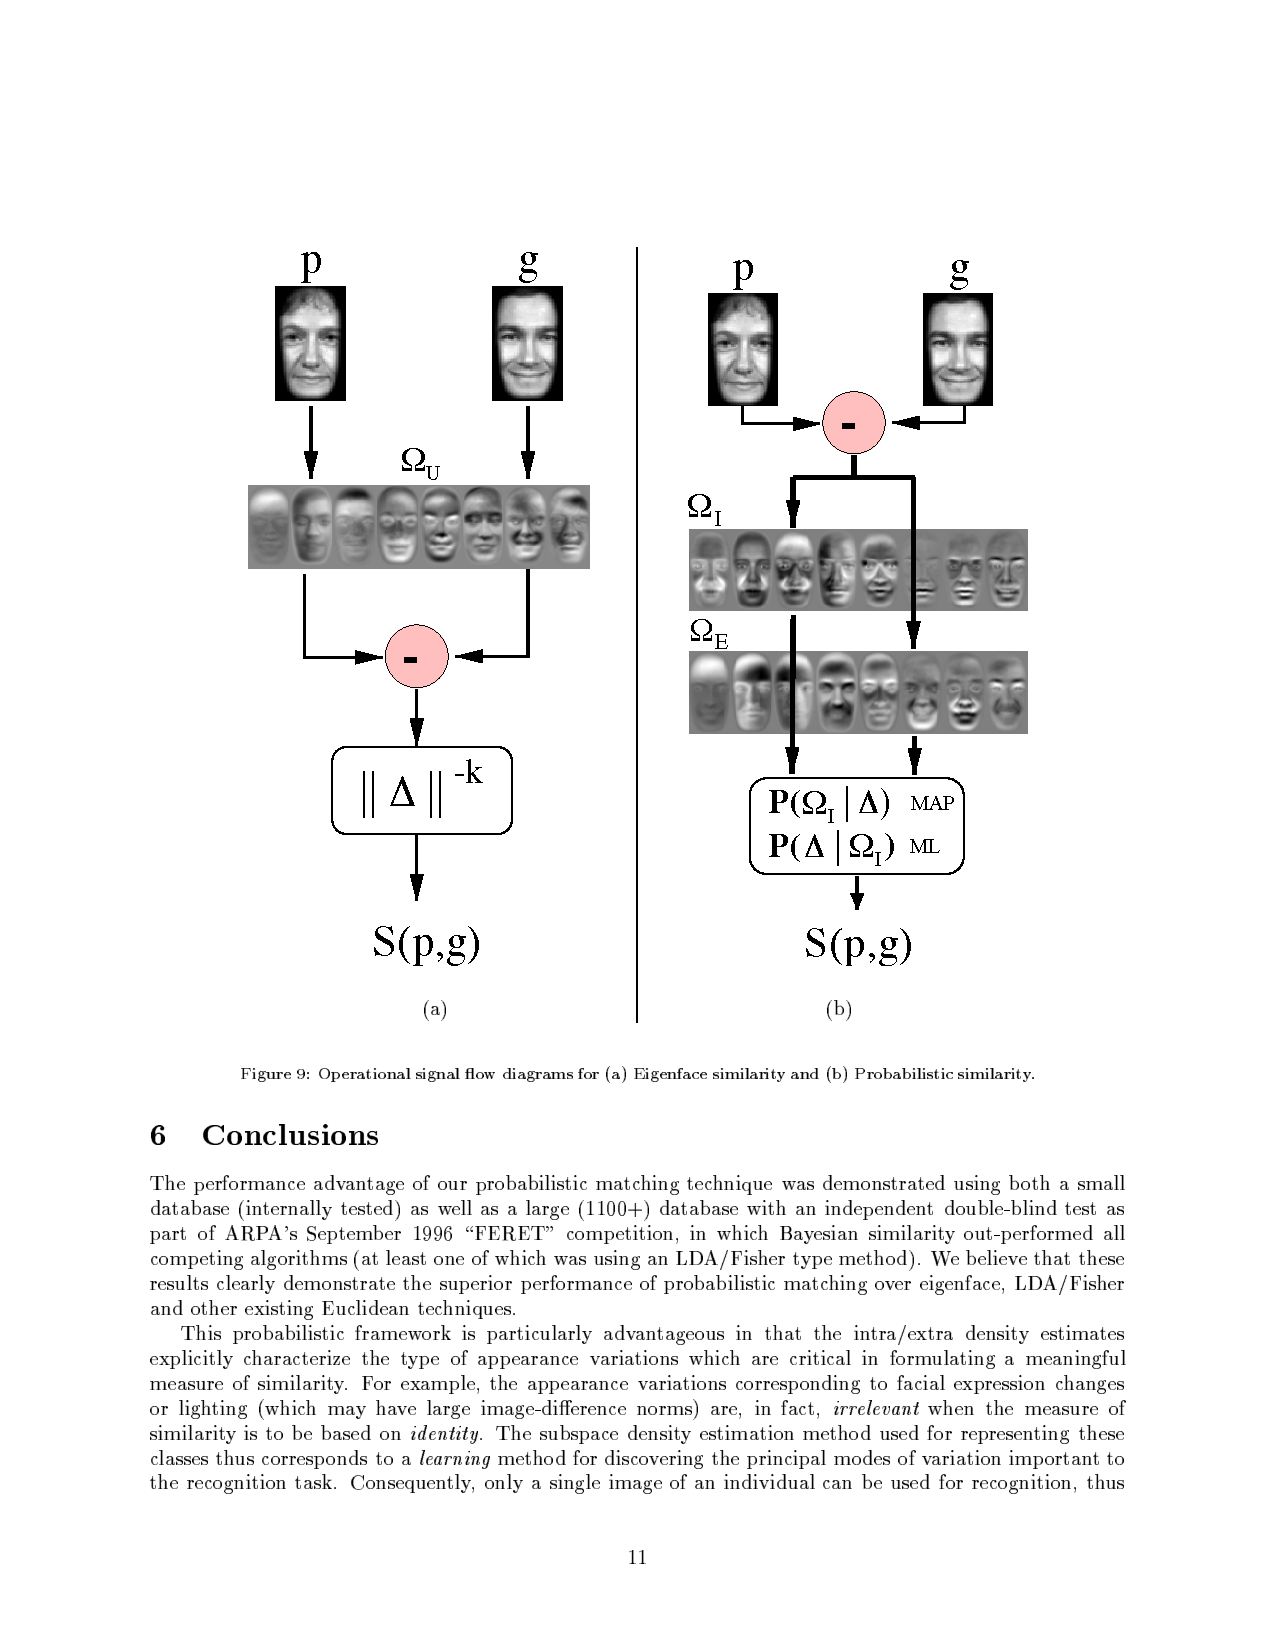
\includegraphics[height=\textheight, trim=1.6in 3.75in 1.6in 1.6in, clip]{Moghaddam13}
\end{figure}
\end{frame}

\begin{frame}
\frametitle{Efficient similarity computation}
\begin{block}{The Problem}
Expensive similarity computation
\begin{itemize}
\pause
\item Subtract the candidate image $I_j$ from the database entry $I_k$.
\pause
\item Project the resulting $\Delta$ onto the principal eigenvectors of both the extrapersonal and intrapersonal Gaussians.
\pause
\item Evaluate the exponentials are plug into Bayes formula.
\pause
\item Repeat for all images in the database
\end{itemize}
\end{block}
\end{frame}

\begin{frame}
\frametitle{Efficient similarity computation}
\begin{block}{The Solution}
Pre-process each image with \emph{whitening} transformations, representing the image as two vectors of whitened subspace coefficients
\pause
\begin{equation}
\mathbf{i}_j=\Lambda_I^{-1/2}V_II_j\ \ \ \ \mathbf{e}_j=\Lambda_E^{-1/2}V_EI_j
\end{equation}
\pause
and evaluating likelihoods is reduced to computing Euclidean distances
\begin{equation}
\begin{split}
P(\Delta|\Omega_E)& = \frac{e^{-1/2}||\mathbf{e_j}-\mathbf{e_k}||^2}{(2\pi)^{D/2}|\Sigma_E|^{1/2}} \\
P(\Delta|\Omega_I)& = \frac{e^{-1/2}||\mathbf{i_j}-\mathbf{i_k}||^2}{(2\pi)^{D/2}|\Sigma_I|^{1/2}}
\end{split}
\end{equation}
\end{block}
\pause
\begin{block}{Question}
What happened to $\hat{P}_{\bar{f}}(\Delta|\Omega)$, $\epsilon^2(\Delta)$, and $p$?
\end{block}
\end{frame}

\begin{frame}
\frametitle{``Dual'' Eigenfaces}
\begin{figure}[H]
\centering
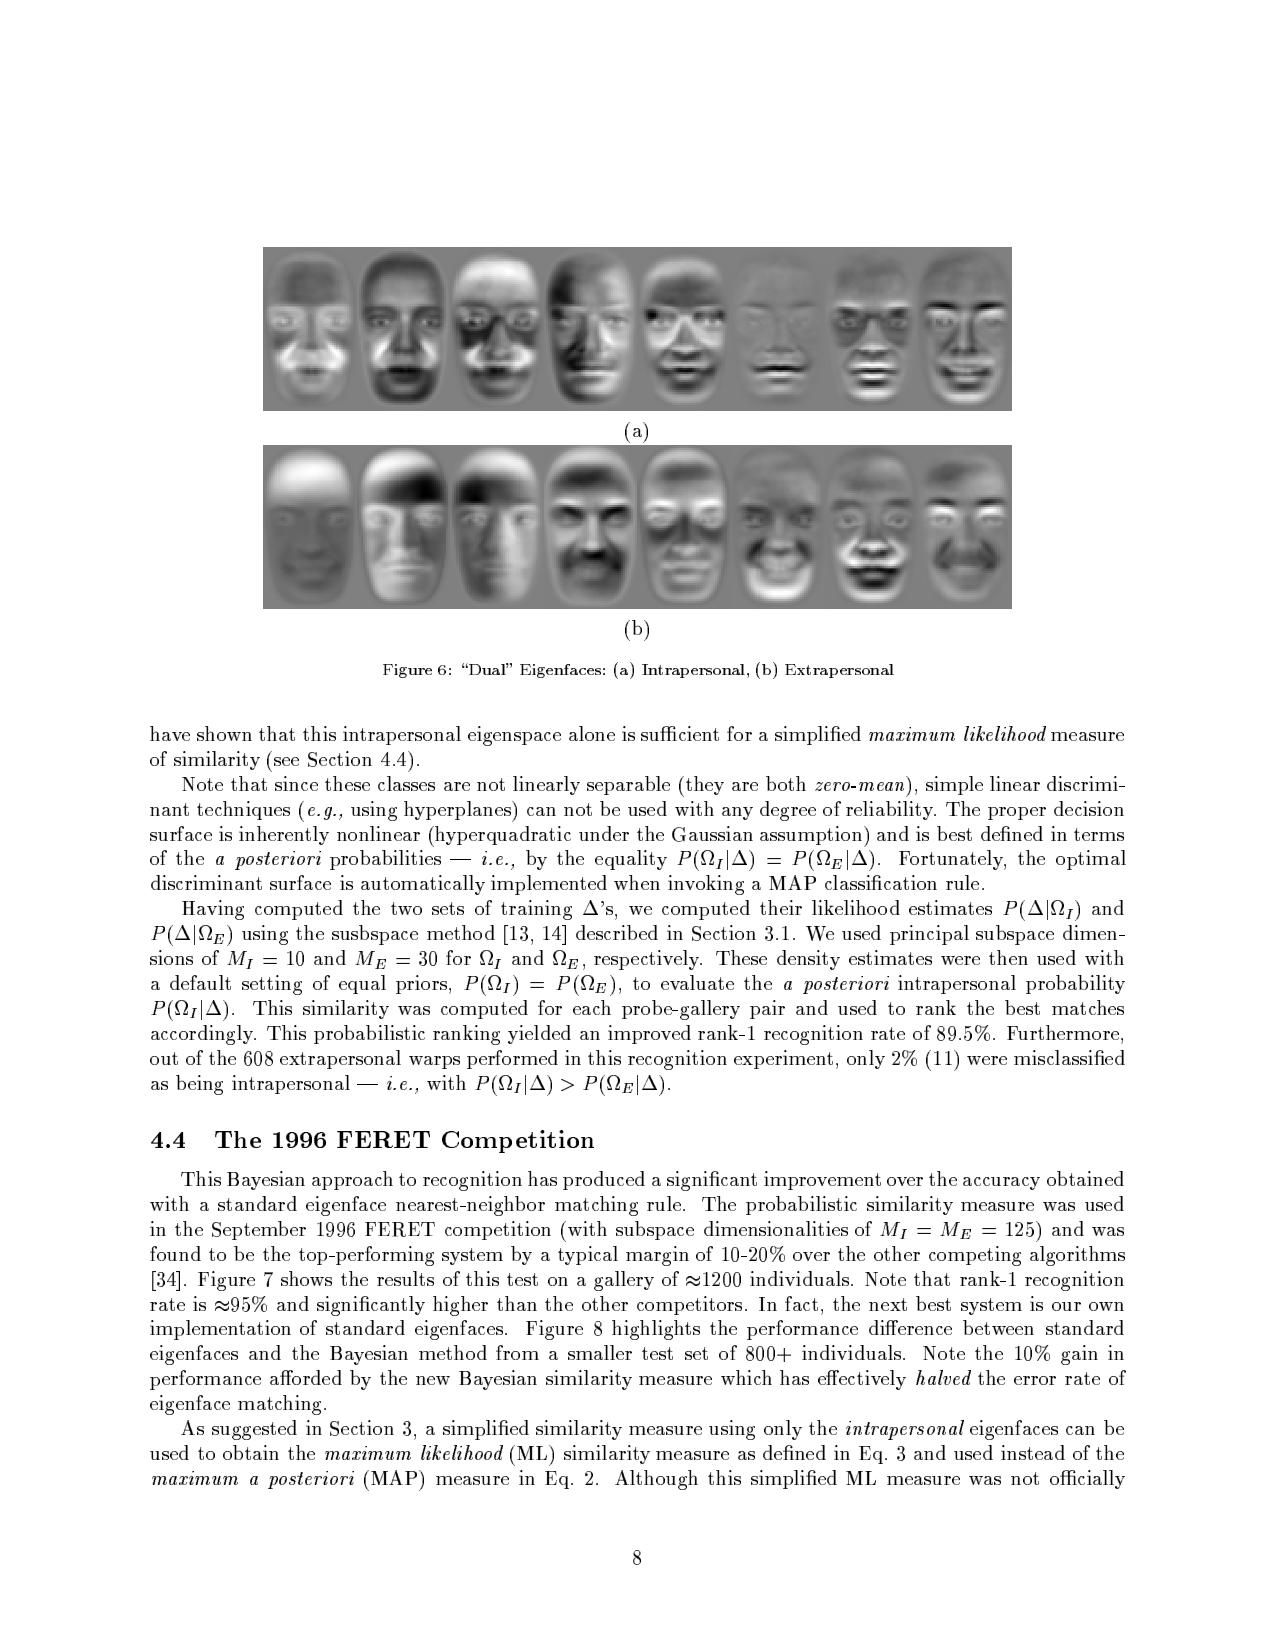
\includegraphics[width=\textwidth, trim=1.6in 6.4in 1.6in 1.6in, clip]{Moghaddam10}
\end{figure}
\end{frame}

\begin{frame}
\frametitle{Results}
\begin{figure}[H]
\centering
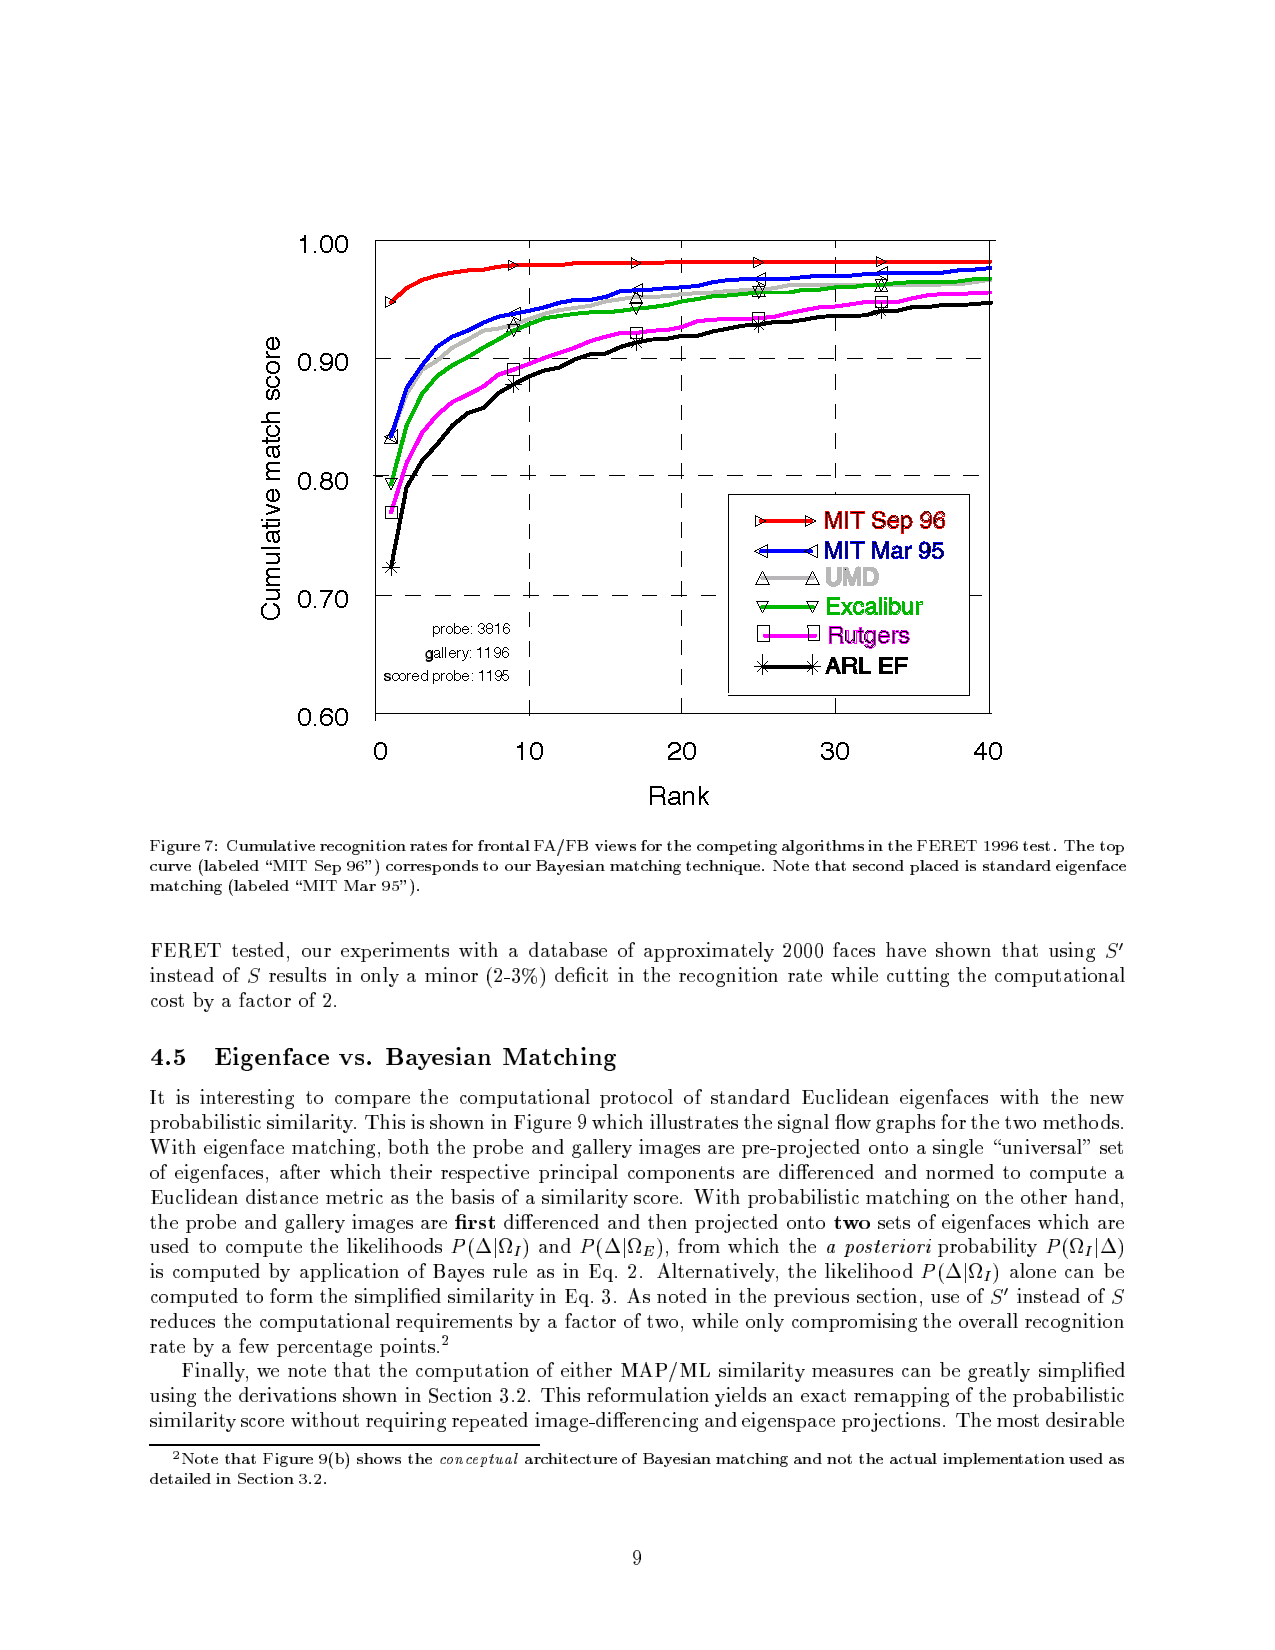
\includegraphics[height=\textheight, trim=1.6in 4.9in 1.6in 1.4in, clip]{Moghaddam11}
\end{figure}
\end{frame}

\section{Probabilistic Models for Inference about Identity}
\begin{frame}
\frametitle{Probabilistic Models for Inference about Identity}
\begin{block}{Abstract}
\begin{itemize}
\item Model the underlying causes for the presentation of a face image.
\pause
\item Function of both the identity (latent identity variables, or LIVs) and other causes.
\pause
\item Consider three increasingly sophisiticated models for face representation with two perspectives taken for each model.
\pause
\item Demonstrate state of the art performance for both frontal face recognition and face recognition under varying pose.
\end{itemize}
\end{block}
\end{frame}

\begin{frame}
\frametitle{Introduction}
\begin{block}{Motivation}
Probabilistic match scores are easier to interpret and combine with scores from other modalities or priors.
\end{block}
\pause
\begin{block}{Model Premises}
\begin{itemize}
\item Face images depend on several interacting factors including identity (signal), pose, illumination, and other nuisance variables.
\pause
\item Image generation is noisy even under good conditions.
\pause
\item There will always be some uncertainty in any estimate of identity.
\pause
\item Recognition tasks need not perform identity estimation, rather they can just answer whether two faces have the \emph{same} identity.
\end{itemize}
\end{block}
\end{frame}

\begin{frame}
\frametitle{Overview}
\begin{block}{General Model}
\begin{equation}
\mathbf{x}_{ij} = f(\mathbf{h}_i, \mathbf{w}_{ij}, \theta) + \epsilon_{ij}
\end{equation}
\pause
\begin{itemize}
\item $\mathbf{x}_{ij}$ is the vectorized data from the $j$th image of the $i$th person.
\pause
\item $\mathbf{h}_i$ is the LIV and is constant for every image of a person.
\pause
\item $\mathbf{w}_{ij}$ is another latent variable representing the viewing conditions (pose, illumination, expression, etc.).
\pause
\item $\theta$ is a vector of model parameters learned during the training phase.
\pause
\item $\epsilon_{ij}$ is a Gaussian noise term used to explain any remaining variation.
\end{itemize}
\end{block}
\end{frame}

\begin{frame}
\frametitle{General Model}
\begin{block}{Two Perspectives}
Assuming that we know the model parameters, $\theta$, how can we then identify if a gallery and probe face match?
\end{block}
\pause
\begin{block}{Joint Perspective}
\begin{itemize}
\item Infer whether two observed images $x_1$ and $x_2$ were generated from the same identity variable $h$.
\pause
\item Deal with uncertainty in $h$ and $w$ by considering all possible values of them. One possible value for each face in the target gallery.
\end{itemize}
\end{block}
\pause
\begin{block}{Class Conditional Perspective}
\begin{itemize}
\item Consider the predictive distribution for the probe image $x_p$ induced by the matching gallery data $x_g$ in each of the models.
\pause
\item "One shot" model generation for each gallery template.
\end{itemize}
\end{block}
\end{frame}

\begin{frame}
\frametitle{Probabilistic LDA}
\begin{block}{Probabilistic LDA}
\begin{itemize}
\item PLDA is to LDA as factor analysis is to PCA.
\pause
\item Seek directions that have maximum discriminability (signal term) while also explicitly modeling within-individual variance.
\pause
\item Model parameters learned using expectation maximization (EM).
\end{itemize}
\end{block}
\pause
\begin{block}{Results}
Authors demonstrate state of the art performance on frontal face identification, clustering, and verification when compared against other recent subspace learning approaches.
\end{block}
\end{frame}

\begin{frame}
\frametitle{Mixtures of PLDAs}
\begin{block}{Mixtures of PLDAs}
Describe the face manifold as a weighted additive mixture of K PLDA distributions.
\pause
Overcomes weaknesses of PLDA:
\pause
\begin{itemize}
\item Unrealistic that the face manifold is well modeled by a linear subspace.
\pause
\item Unlikely that the noise distribution is identical at each point in space.
\end{itemize}
\pause
Clusters also learned by EM. Interestingly, when K=2, the clusters separate men from women.
\end{block}
\pause
\begin{block}{Results}
Inconclusive improvement when compared against PLDA. Hindered by a lack of training data.
\end{block}
\end{frame}

\begin{frame}
\frametitle{Tied PLDA}
\begin{block}{Tied PLDA}
\begin{itemize}
\item Need a more powerful technique for matching images across large pose changes.
\pause
\item In "tied" models, two or more viewing conditions are compared by assuming that they have a common underlying LIV, but different generation processes.
\pause
\item Similar learning process to MixPLDA except with an additional M-Step in the learning process where clusters are updated using only the data known to come from these clusters.
\end{itemize}
\end{block}
\pause
\begin{block}{Results}
Considerably improves off-pose face recognition performance. Does not improve frontal face recognition accuracy.
\end{block}
\end{frame}

\section{Bayesian Face Revisited: A Joint Formulation}
\begin{frame}
\frametitle{Bayesian Face Revisited: A Joint Formulation}
\begin{block}{Abstract}
\begin{itemize}
\item Revist the classic Bayesian face recognition method.
\pause
\item Replace the "difference" formulation with a "joint" formulation.
\pause
\item Solve the model using EM-like learning algorithm.
\pause
\item Demonstrate high accuracy on Labeled Faces in the Wild (LFW).
\end{itemize}
\end{block}
\end{frame}

\begin{frame}
\frametitle{General Idea}
\begin{figure}[H]
\centering
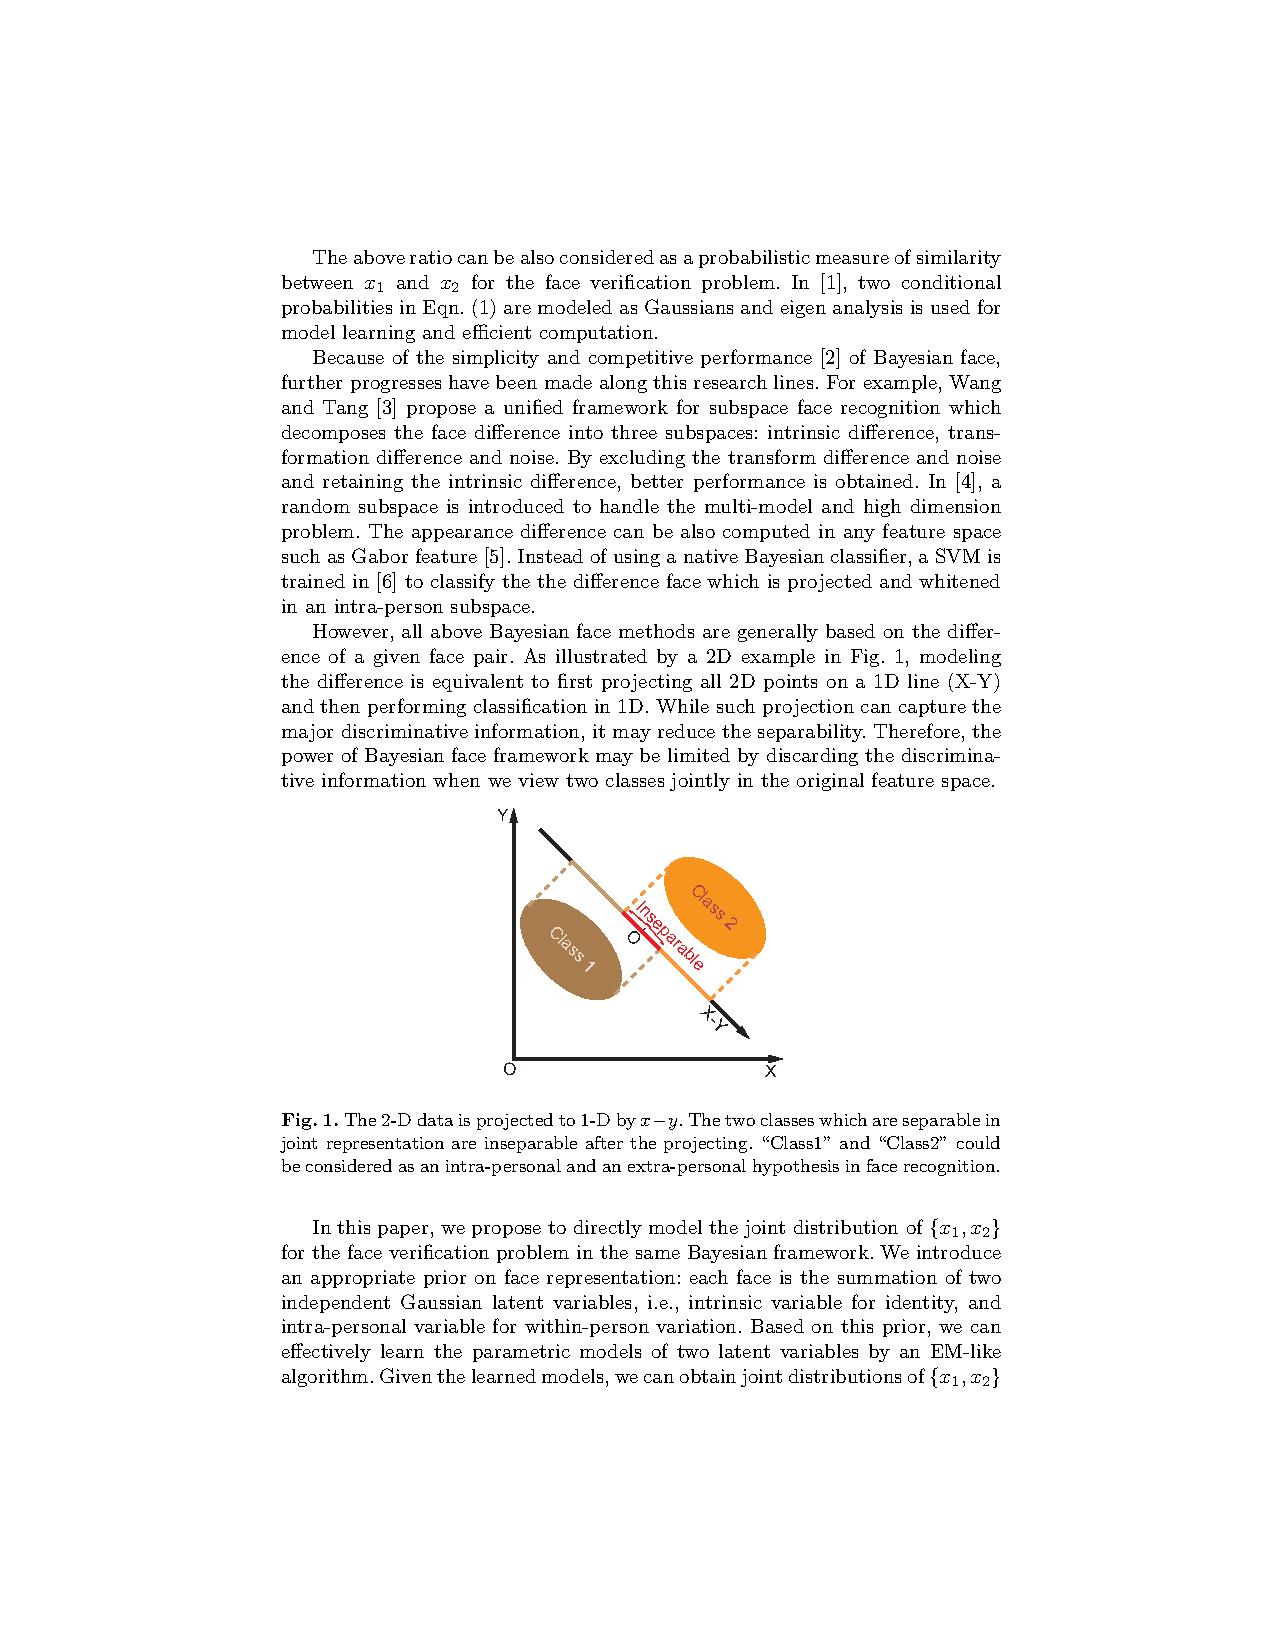
\includegraphics[height=\textheight, trim=3.25in 3.4in 3.25in 5.4in, clip]{Chen2}
\end{figure}
\end{frame}

\begin{frame}
\frametitle{Model Formulations}
\begin{block}{Naive Model}
\begin{itemize}
\item Directly model the joint distribution of $\{x_1,x_2\}$ as a Gaussian.
\pause
\item Moderately better than conventional Bayesian face.
\pause
\item Insufficient training samples to compute reliable second order statistics.
\end{itemize}
\end{block}
\pause
\begin{block}{Joint Model}
\begin{itemize}
\item Face representation $x = \mu + \epsilon$.
\begin{itemize}
\item $x$ is mean subtracted image
\item $\mu$ is identity
\item $\epsilon$ is face variation.
\pause
\item $mu$ and $\epsilon$ are assumed to be Gaussian and \emph{independent}.
\pause
\item Restricts the shape of the joint covariance matrix.
\end{itemize}
\end{itemize}
\end{block}
\end{frame}

\begin{frame}
\frametitle{Observations}
\begin{block}{Model Learning}
Objective function appears to have very good "convex" properties as the resulting accuracy is relatively invariant to the initial parameter estimation.
\end{block}
\pause
\begin{block}{Connection with metric learning}
$(x_1-x_2)^TM(x_1-x_2)$ versus $x_1^TAx_1+x_2^TAx_2-2x_1^TGx_2$
\end{block}
\pause
\begin{block}{Connection with LDA and PLDA}
Each dimension is treated equally \emph{unlike} LDA/PLDA where the descriminiability of each new dimension decreases.
\end{block}
\pause
\begin{block}{Reference Based Methods}
Reference-based methods represent a face by its similarites to a set of reference faces. The joint model can be considered as a kind of probabilistic reference based method, with infinite references, but under Gaussian assumptions.
\end{block}
\end{frame}

\begin{frame}
\frametitle{Results}
\begin{figure}[H]
\centering
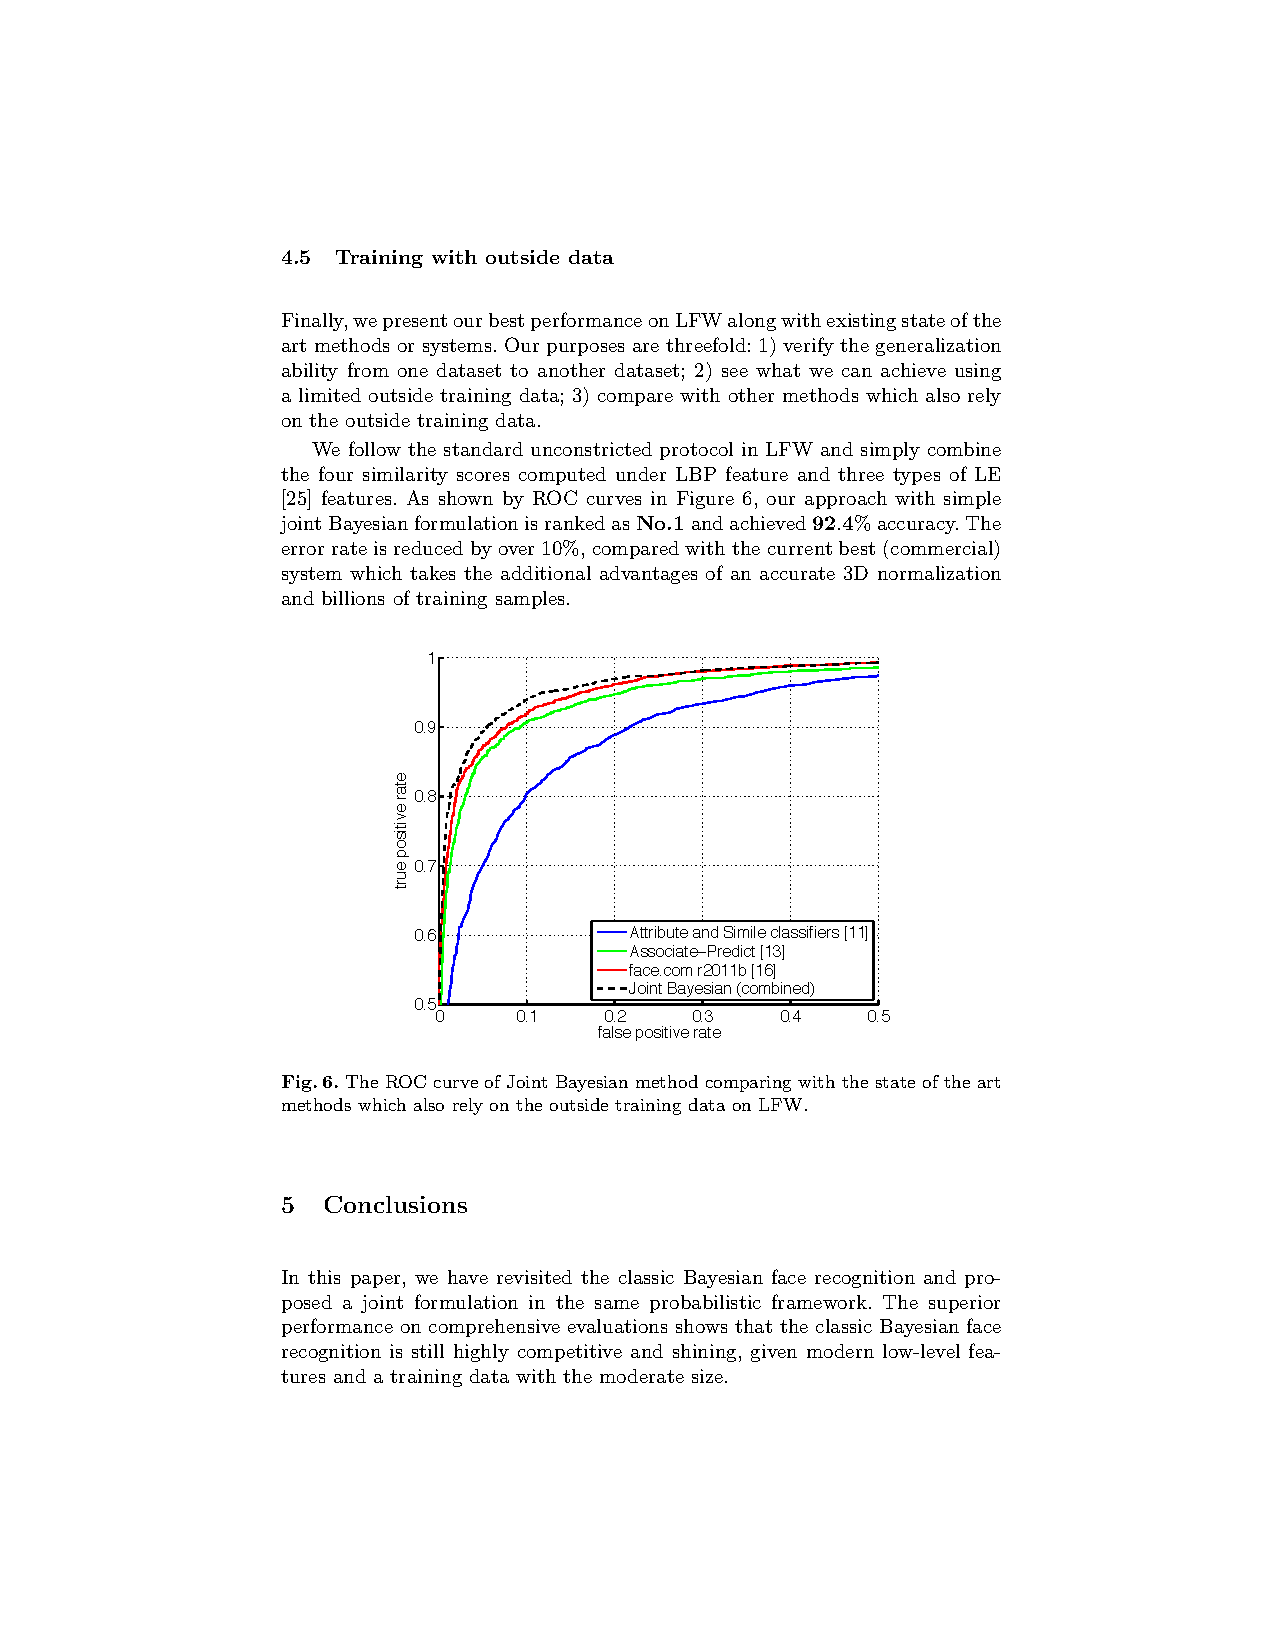
\includegraphics[height=\textheight, trim=2.25in 3.5in 2.25in 4.2in, clip]{Chen13}
\end{figure}
\end{frame}

\begin{frame}
\centerline{The End!}
\end{frame}

% End of slides
\end{document}